\documentclass[../AnalysisNoteJBuxton.tex]{subfiles}
\begin{document}

\subsubsection{\texorpdfstring{K$^{0}_{S}$}{TEXT} Reconstruction}
\label{K0sReconstruction}

The following cuts were used to select good K$^{0}_{S}$ candidates:

\begin{enumerate}
 \item{Pion Daughter Cuts}
 \begin{enumerate}
  \item $|\eta| < 0.8$
  \item SetTPCnclsDaughters(80)
  \item SetStatusDaughters(AliESDtrack::kTPCrefic)
  \item SetMaxDcaV0Daughters(0.3)
  \item $p_{T} >$ 0.15
  \item DCA to prim vertex $>$ 0.3
 \end{enumerate}

 \item K$^{0}_{S}$ Cuts
 \begin{enumerate}
  \item $|\eta| < 0.8$
  \item $p_{T} > 0.2$
  \item $m_{PDG} -$ 13.677 MeV $< m_{inv} < m_{PDG} +$ 2.0323 MeV
  \item Cosine of pointing angle $>$ 0.9993
  \item OnFlyStatus = false
  \item Decay Length $<$ 30 cm
 \end{enumerate}  
 
\end{enumerate}

\begin{figure}[h]
  \centering
  \includegraphics[width=100mm]{3_DataSelection/Figures/MassAssHypotheses/canMassAssLamHypCompare_LamK0_wNoMisID.pdf}
  \caption[$\Lambda$ contamination in K$^{0}_{S}$ collection]{Mass assuming $\Lambda$-hypothesis for V0 candidates passing all K$^{0}_{S}$ cuts, i.e. assume the daughters are $p^{+}\pi^{-}$ instead of $\pi^{+}\pi^{-}$.
  The peak around $m_{inv} = $ 1.115 GeV/c$^{2}$ contains misidentified $\Lambda$ particles in our K$^{0}_{S}$ collection.
  If one simply cuts out the entire peak, some good K$^{0}_{S}$ particles will be lost.  Ideally, the K$^{0}_{S}$ selection and $\Lambda$($\bar{\Lambda}$) misidentification cuts can be selected such that the peak is removed from this plot while leaving the distribution continuous.
  Also note, the excess around 1.65 $<$ $m_{inv}$ $<$ 2.1 GeV/c$^{2}$ shows misidified $\bar{\Lambda}$ particles in our K$^{0}_{S}$ collection.}
  \label{fig:MassAssLamHyp}
\end{figure}


\begin{figure}[h]
  \centering
  \includegraphics[width=100mm]{3_DataSelection/Figures/MassAssHypotheses/canMassAssALamHypCompare_LamK0_wNoMisID.pdf}
  \caption[$\bar{\Lambda}$ contamination in K$^{0}_{S}$ collection]{Mass assuming $\bar{\Lambda}$-hypothesis for V0 candidates passing all K$^{0}_{S}$ cuts, i.e. assume the daughters are $\pi^{+}\bar{p}^{-}$ instead of $\pi^{+}\pi^{-}$.  Similar to Figure \ref{fig:MassAssLamHyp}}
  \label{fig:MassAssALamHyp}
\end{figure}

As can be seen in Figures \ref{fig:MassAssLamHyp} and \ref{fig:MassAssALamHyp}, some misidentified $\Lambda$ and $\bar{\Lambda}$ particles contaminate our K$^{0}_{S}$ sample.
Figure \ref{fig:MassAssLamHyp} shows the mass assuming $\Lambda$-hypothesis for V0 candidates passing all K$^{0}_{S}$ cuts, i.e. assume the daughters are $p^{+}\pi^{-}$ instead of $\pi^{+}\pi^{-}$.
Figure \ref{fig:MassAssALamHyp} is similar, but shows the mass assuming $\bar{\Lambda}$ hypothesis for the same K$^{0}_{S}$ collection, i.e. assume the daughters are $\pi^{+}\bar{p}^{-}$ instead of $\pi^{+}\pi^{-}$.
The $\Lambda$ contamination can be seen in Figure \ref{fig:MassAssLamHyp}, and the $\bar{\Lambda}$ contamination in Figure \ref{fig:MassAssALamHyp}, in the peaks around $m_{inv}$ = 1.115 GeV/c$^{2}$.
Additionally, the $\bar{\Lambda}$ contamination is visible in Figure \ref{fig:MassAssLamHyp}, and the $\Lambda$ contamination visible in Figure \ref{fig:MassAssALamHyp}, in the region of excess around 1.65 $<$ $m_{inv}$ $<$ 2.1 GeV/c$^{2}$.
This is confirmed as the number of misidentified $\Lambda$ particles in the sharp peak of Figure \ref{fig:MassAssLamHyp} (misidentified $\bar{\Lambda}$ particles in the sharp peak of Figure \ref{fig:MassAssALamHyp}) approximately equals the excess found in the 1.65 $<$ $m_{inv}$ $<$ 2.1 GeV/c$^{2}$ region of Figure \ref{fig:MassAssALamHyp} (Figure \ref{fig:MassAssLamHyp}).

The peak around $m_{inv} = $ 1.115 GeV/c$^{2}$ in Figure \ref{fig:MassAssLamHyp} (Figure \ref{fig:MassAssALamHyp})contains both misidentified $\Lambda$ ($\bar{\Lambda}$) particles and good K$^{0}_{S}$.
If one simply cuts out the entire peak, some good K$^{0}_{S}$ particles will be lost.  Ideally, the K$^{0}_{S}$ selection and $\Lambda$($\bar{\Lambda}$) misidentification cuts can be selected such that the peak is removed from this plot while leaving the distribution continuous.
To attempt to remove these $\Lambda$ and $\bar{\Lambda}$ contaminations without throwing away good K$^{0}_{S}$ particles, the following misidentification cuts are imposed; a K$^{0}_{S}$ candidate is rejected if all of the following criteria are satisfied:
\begin{itemize}
 \item $|m_{inv, \ \Lambda(\bar{\Lambda}) \ Hypothesis} - m_{PDG,\ \Lambda(\bar{\Lambda})}| < $ 9.0 MeV/c$^{2}$
 \item Positive daughter passes $p^{+}$($\pi^{+}$) daughter cut implemented for $\Lambda$($\bar{\Lambda}$) reconstruction
 \item Negative daughter passes $\pi^{-}$($\bar{p}^{-}$) daughter cut implemented by $\Lambda$($\bar{\Lambda}$) reconstruction
\end{itemize} 


\begin{figure}[h]
  \centering
  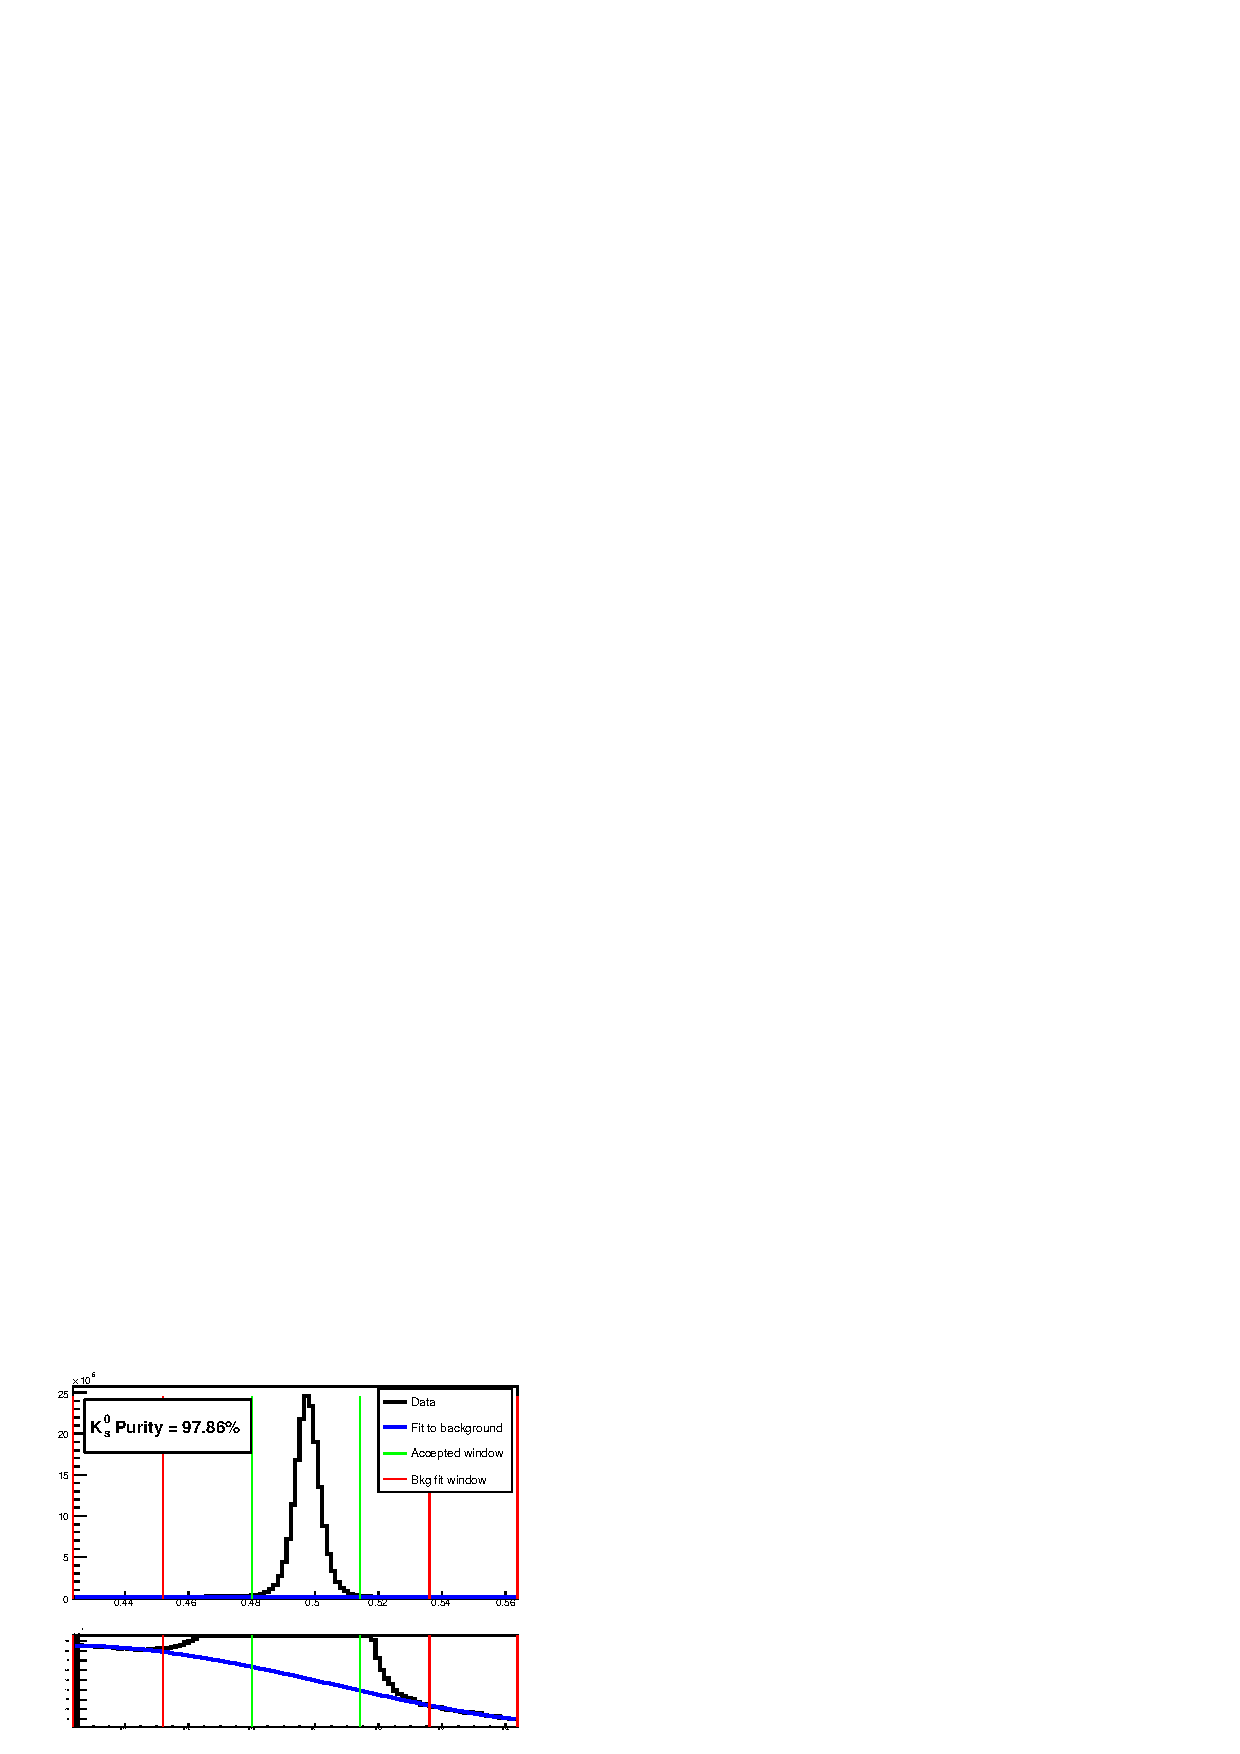
\includegraphics[width=100mm]{3_DataSelection/Figures/K0Purity_LamK0.pdf}
  \caption[K$^{0}_{S}$ Purity]{K$^{0}_{S}$ Purity}
  \label{fig:K0Purity}
\end{figure}

\end{document}